\begin{taged}{人物}
\section{2022-12-06 纪念江泽民}
\end{taged}

前国家主席江泽民同志,于2022年11月30日因病去世。

\begin{figure}[htbp]
    \centering
    \begin{minipage}{6cm}
        \centering
        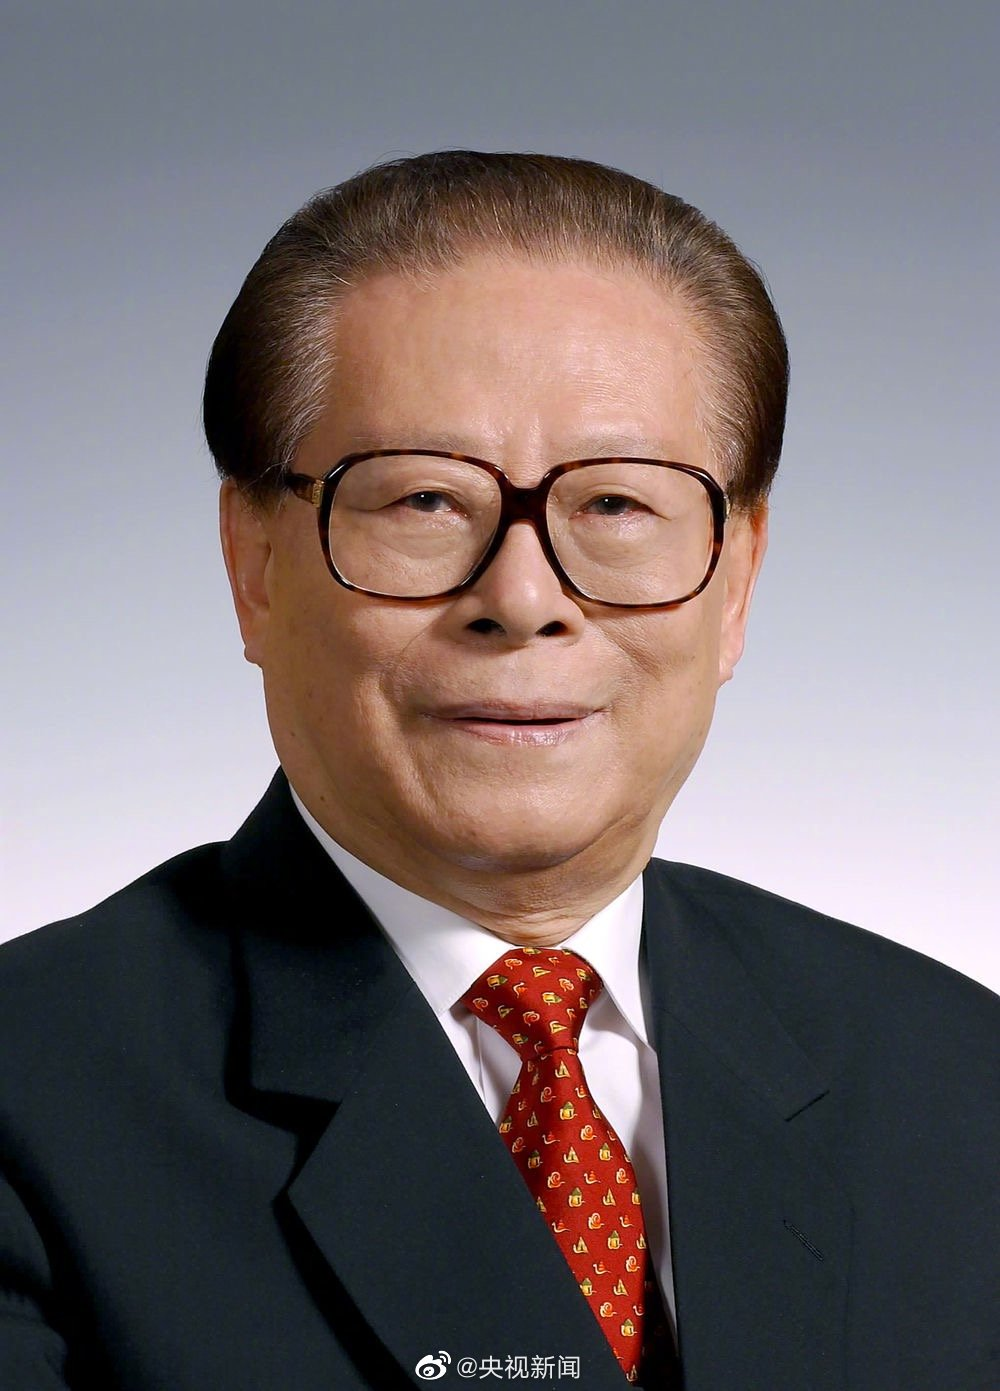
\includegraphics[width=6cm]{pic/江泽民.jpg}
        \caption*{江泽民}
    \end{minipage}
    \quad
    \begin{minipage}{6cm}
        \centering
        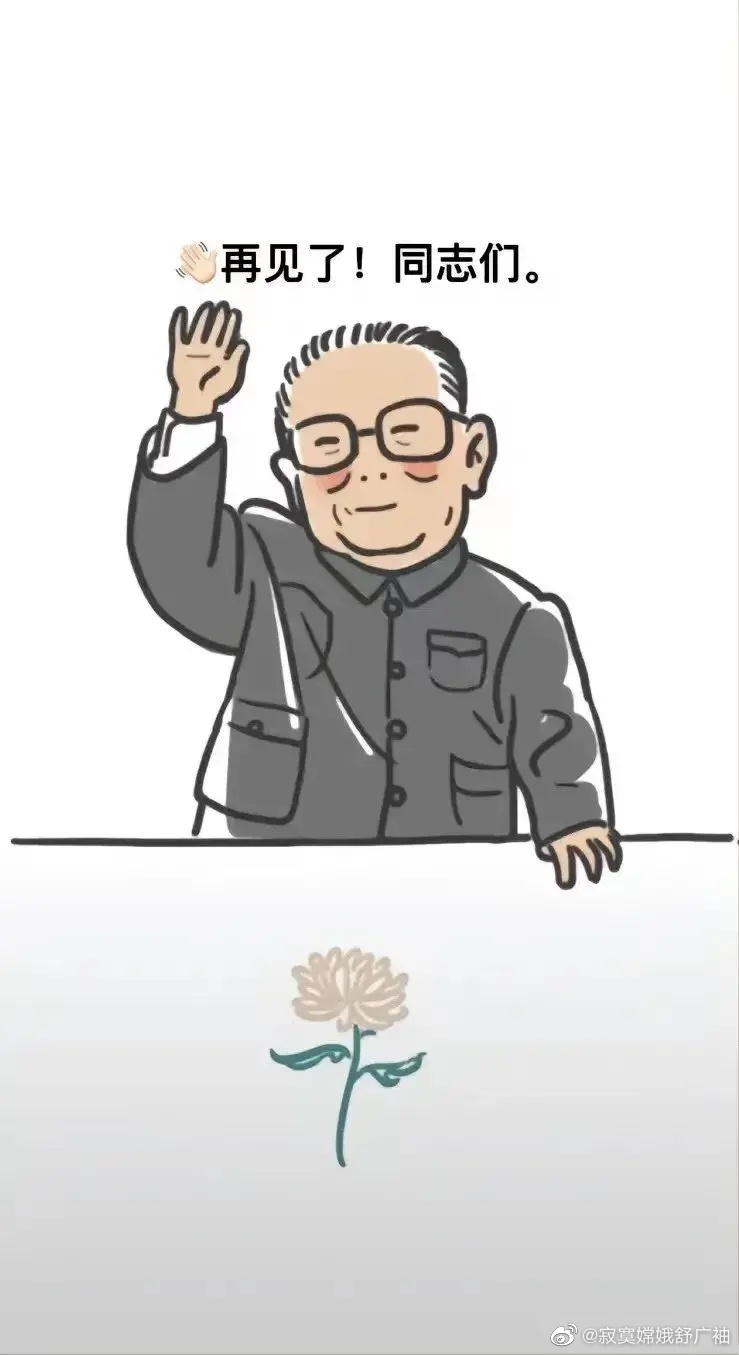
\includegraphics[width=4.5cm]{pic/再见了,同志们.jpg}
        \caption*{再见了,同志们}
    \end{minipage}
\end{figure}

今天上午,去社区参加集体活动:观看直播的江泽民同志追悼大会。

江泽民同志是我党的第三代中央领导集体的核心。党的十三届四中全会以后,在国内外形势十分复杂、世界社会主义出现严重曲折的严峻考验面前,江泽民带领党的中央领导集体,紧紧依靠全党全军全国各族人民,捍卫了中国特色社会主义伟大事业,成功把中国特色社会主义推向二十一世纪,建立了永不磨灭的功勋,赢得了全党全军全国各族人民衷心爱戴和国际社会广泛赞誉。

他在中国改革开放关键时期发挥着中流砥柱作用,为中国现代化和走向世界奠定了坚实的基础。而他却自我评价为“干了这十几年也没有什么别的,大概三件事”\footnote{见“素材”目录中的:江泽民自我评价.mp4}:

一、确立了社会主义市场经济

二、把邓小平理论写入党章

三、提出“三个代表”

除了以上三点之外,他值得称赞的地方还有\footnote{https://weibo.com/5476743904/MhtiW9vF7}:

\begin{itemize}[nosep, left=\parindent]
    \item 禁止军队经商的远见和魄力;
    \item 捣毁邪教的决绝和勇气;
    \item 继承收回香港澳门的历史责任;
    \item 加入WTO推动经济发展;
    \item 98抗洪前线的身影;
    \item 应对银河号的忍辱负重;
    \item 抵挡金融风暴的手段和决心。
\end{itemize}

江泽民同志同我们永别了。他的英名、业绩、思想、风范将永载史册,世世代代铭刻在人民心中。

\centering\Huge 江泽民同志永垂不朽!
